\chapter{Introduction}
\pagenumbering{arabic}


\section{Sequencing}\label{sec:sequencing}
Since 1869 and the discovery of ``nuclein'' by \href{https://books.google.fr/books?id=YJRTAAAAcAAJ&pg=PA456&redir_esc=y#v=onepage&q&f=false}{F.~\textsc{Miescher}}, we have come to understand that \gls{dna} is the basis of every living organism on Earth.
It is a code composed of four letters (nucleotides).
In order to read this code and maybe be able to decipher it, new technologies had to be invented.

In the early 1970s, R.~\textsc{Wu}, R.~\textsc{Padmanabhan} and later \href{https://www.ncbi.nlm.nih.gov/pubmed/271968}{F.~\textsc{Sanger}} created a process called sequencing to read the nucleotides in a \gls{dna} molecule.
In 1977, F.~\textsc{Sanger} and his team performed the first complete genome sequencing (\href{https://www.ncbi.nlm.nih.gov/pubmed/870828}{bacteriophage \textphi X174}).
In 2003, the International Human Genome Sequencing Consortium announced that the Human genome had been essentially sequenced.

In the next years appeared new technologies called \gls{ngs} that revolutionized genome research.
These technologies, especially \href{http://www.illumina.com/}{Illumina\ttfamily\tiny\raise2ex\hbox{\textregistered}}, will be discussed in more detail in Section~\ref{sec:ngs}.
They have allowed the researchers to obtain sequences much faster than what was possible before and at a fraction of the price.
This has contributed to the more widespread use of \gls{dna} sequencing.
Nowadays, medical practionners use it more and more commonly to clarify the diagnostic of genetic pathologies and\slash\hspace{0pt}or to predict the risks of developing one.

Thanks to \gls{ngs}, we are now able to ``read the Human code'' relatively easily; deciphering it however is still a work in progress.
One of the processes used to understand it is to compare the genomes of different individuals.
This involves aligning the sequences and identifying mutations that would explain the differences in the observed phenotypes.
The alignment could theoretically be done by hand but as the Human genome is composed of around three billion base pairs, it would be a rather tedious task.
And so, programs have been developed to perform this task.


\section{Basic Local Alignment Search Tool (BLAST)}\label{sec:blast}
\begin{wrapfigure}[3]{l}{0.09\textwidth}
    \vspace{-1.2em}
    
\includegraphics[width=0.1\textwidth]{img/blast}
\end{wrapfigure}

\acrshort{blast} is the most widely known sequence alignment software. It has been developed in 1990 by S.~\textsc{Altschul} at the \gls{ncbi}~\cite{Altschul1990}. Two formats are available, as a web tool on the \href{http://blast.ncbi.nlm.nih.gov/Blast.cgi}{\gls{ncbi} website} and as a command-line tool in \href{ftp://ftp.ncbi.nlm.nih.gov/blast/executables/blast+/LATEST/}{BLAST\texttt{+} package}.
\gls{blast}, as its name suggests, performs alignments between two biological sequences (nucleotide or protein).
The comparison can only be done on primary structures (raw sequences).
There is always at least two sequences: a query and a reference.
It can work with one or several query sequences and one or several references.

\gls{blast} is a local aligner, meaning that it searches for sequence homology by matching the reference with small parts of the query instead of the whole sequence.
Its process can be decomposed into six main steps:
\begin{enumerate}
    \item The query sequence is cut into overlapping subsequences called ``words'' or ``seeds''.
    The cut is dependent on the length of the words generated (\texttt{word\_size}).
    Example: if the query is \texttt{AATGCATCGC} and the \texttt{word\_size} is 8, the resulting subsequences will be \texttt{AATGCATC}, \texttt{ATGCATCG} and \texttt{TGCATCGC}.
    All the words generated are recorded in a dictionary.
    \item A neighborhood of potential words is created around each of the subsequences.
    This neighborhood is constituted to get around the fact that there may be mutations, and so mismatches, between the subsequence and the reference.
    \gls{blast} generates a list of all the words possible considering the \texttt{word\_size}.
    In our example, this would mean $4^8$ words.
    Most of these words are irrelevant as the number of mutations needed to generate them would be too great.
    To filter them, \gls{blast} uses a matrix of similarity in which a determined score is given for matches and mismatches.
    Each word in the list is compared with the subsequence generated in step 1 and, using the matrix, an homology score is generated for each.
    Only the words with a score higher than a given threshold are kept.
    \item The words are tested for matches against the reference.
    \gls{blast} tries to find a perfect match between each remaining word of the neighborhood and the reference.
    \item The elongation of the seed:
    When a match is found, the word, now called a seed, is elongated in both direction.
    Each elongation operation modifies the homology score based on the matrix of similarity.
    The process continues until the score is lower than the given threshold.
    The alignment constituted is called a \acrfull{hsp}.
    \item E-value:
    \gls{blast} then calculates the relevancy of each \gls{hsp} (E-value).
    If, given a threshold, the \gls{hsp} is not found statistically significant, it will be discarded.
    \item Output of the results.
    All the passing alignments are printed in a report.
\end{enumerate}


\section{Next Generation Sequencing (NGS)}\label{sec:ngs}
As we have seen in Section~\ref{sec:sequencing}, around the mid-2000s, the second generation sequencers, commonly called \gls{ngs}, have considerably increased the throughput compared with the first generation ones (\textsc{Sanger} sequencers). They allow the researchers to conceive large-scale projects and consider new applications.
\gls{ngs} comprises different technologies that share the same goal: to obtain a genome sequence fast, with as few errors as possible and for a low cost.
These technologies are:

\begin{itemize}
    \item Pyrosequencing (\href{http://www.454.com/}{454 Life Sciences, Roche}),
    \item Polymerase based sequence by synthesis (\href{http://www.illumina.com/}{Illumina\ttfamily\tiny\raise2ex\hbox{\textregistered}}),
    \item Ligation based sequencing (SOLiD\texttt{\tiny\raise2ex\hbox{\texttrademark}}) (\href{http://www.appliedbiosystems.com/absite/us/en/home.html}{Applied Biosystems\texttt{\tiny\raise2ex\hbox{\texttrademark}}, Thermo Fisher}).
\end{itemize}

They all have their advantages and disadvantages in term of speed, accuracy and cost.
Recently, new sequencers coined as ``third generation sequencers'' have appeared:
\href{http://www.pacificbiosciences.com/}{PacBio\ttfamily\tiny\raise2ex\hbox{\textregistered}} from Pacific Bioscience and \href{https://nanoporetech.com/products-services/minion-mki}{MinION\ttfamily\tiny\raise2ex\hbox{\texttrademark}} from Oxford Nanopore Technologies.

As the experiments proposed in this report are based on data acquired with \href{http://www.illumina.com/}{Illumina\ttfamily\tiny\raise2ex\hbox{\textregistered}} technology, we will now explain its basics.
\pagebreak

\begin{wrapfigure}[3]{l}{0.13\textwidth}
    \vspace{-1.9em}
    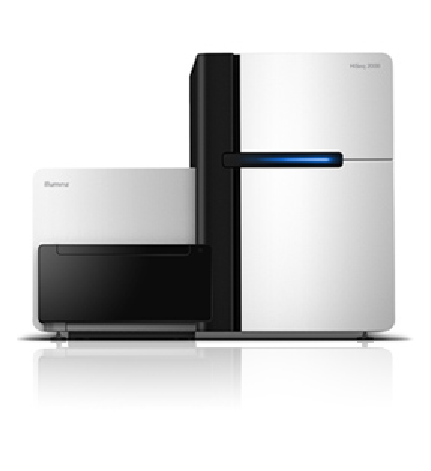
\includegraphics[width=0.15\textwidth]{img/illumina}
\end{wrapfigure}

Illumina\texttt{\tiny\raise2ex\hbox{\textregistered}}'s sequence by synthesis is currently the most used \gls{ngs} technology worldwide. It is based upon the reading of fluorescent markers as the nucleotides on which they are fixed are used by the polymerase to synthesize a copy of the template. The first sequencer to use this technology was the Genome Analyzer produced by Solexa in 2006. \href{http://www.illumina.com/}{Illumina\ttfamily\tiny\raise2ex\hbox{\textregistered}}, now owner of the technology, commercializes it into four series of sequencers: MiSeq, NextSeq, HiSeq and HiSeq X.

The sequencing is composed of four main steps~\cite{Illumina2008}:
\begin{itemize}
    \item Library preparation:
    The \gls{dna} is cut into small fragments (200--500 base pairs) and adapters are fixed on their extremities.
    \item Clustering:
    Each fragment is hybridized onto the flow cell and amplified to form a cluster by a process called bridge amplification.
    To put it simply, it is a \gls{pcr} that uses the special coating of the flow cell to make copies of the fragment and keep them attached to the surface. This way, the multiple copies of each fragment are located on a particular region of the cell. This is done in order to get a clear signal during the sequencing.
    \item Sequencing:
    First, a probe is fixed on the free extremity of each fragment. Then, fluorescently labeled nucleotides are added with the polymerase.
    Each nucleotide is assigned a specific wavelength.
    Each cycle consists in the extension, one nucleotide at a time, of the strand based on the probe. The process is performed as follows:
    \begin{itemize}
        \item The polymerase puts the corresponding nucleotide at the end of the sequence.
        \item The reaction is stopped due to the label.
        \item The fluorescence is detected by a camera.
        \item The label is cut. A new cycle can begin.
    \end{itemize}
    Depending on the sequencer, there can be a maximum of 150 to 300 cycles, thus producing reads with a maximum length of 150 to 300 bases.
    The reads are then written into a fastQ file. We will talk more about this file format in Section~\ref{sec:shortReads}.

    \item Data analysis:
    It consists in, firstly, the alignment of the reads to a reference and then the identification of the differences and their biological meaning.
\end{itemize}

The sequencing can be done in two different modes: single-end and paired-end.
In single-end, each \gls{dna} fragment is read on one end.
In paired-end, it is read on both ends, thus increasing the probability that the fragment will be well aligned on the reference.
In that case, the clustering and sequencing steps are repeated for the complementary strand.
A representation of the position of the reads in paired-end sequencing is shown on figure~\ref{fig:pairedEndSeq}.
In common usage, the read associated with the current read is called its ``mate''.

\begin{figure}[h]
    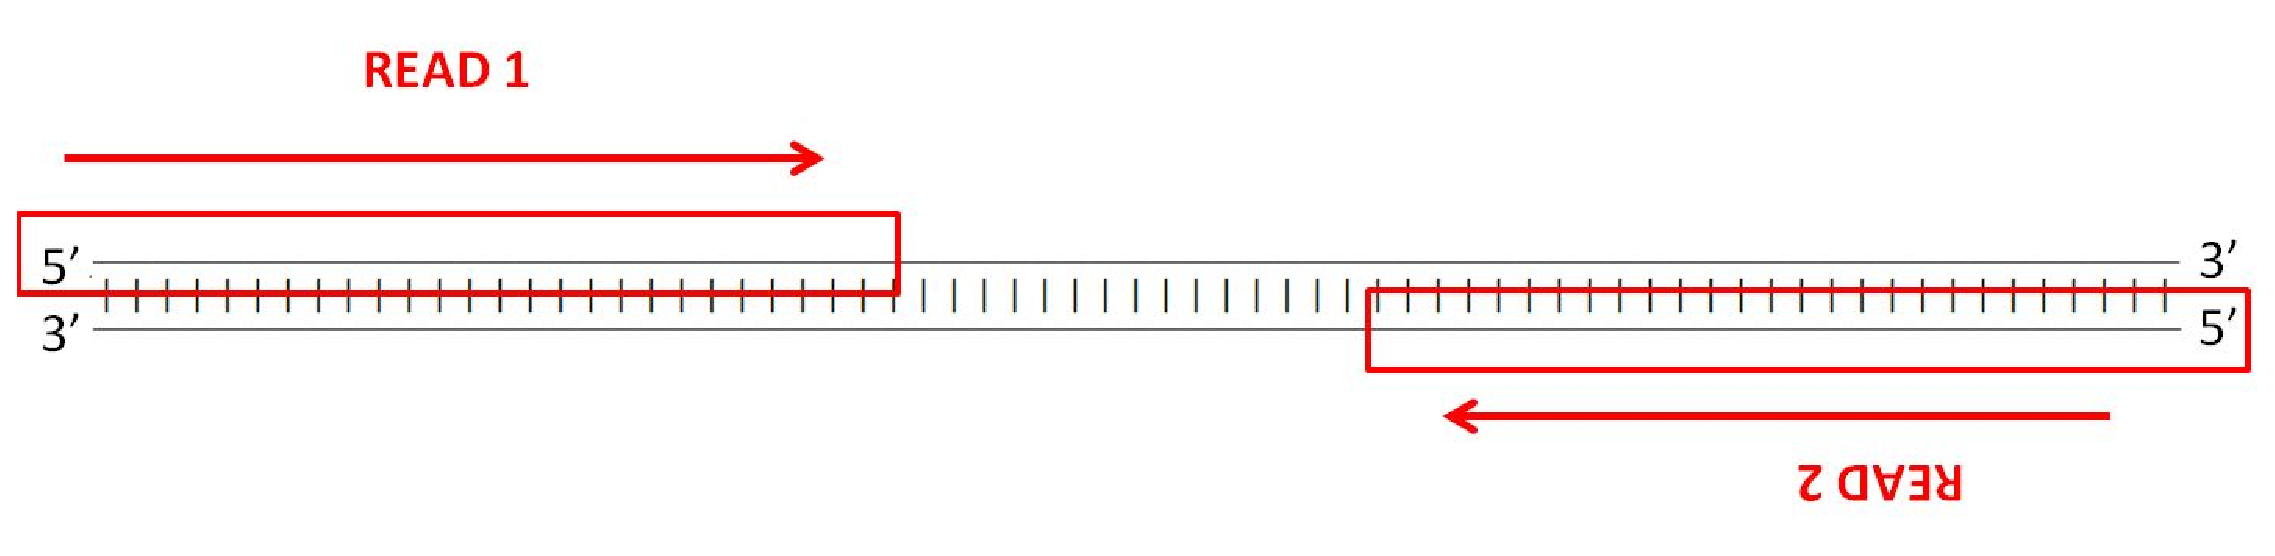
\includegraphics[width=\textwidth]{img/pairedEnd}
    \caption{Representation of paired-end sequencing.}\label{fig:pairedEndSeq}
\end{figure}

\href{http://www.illumina.com/}{Illumina\ttfamily\tiny\raise2ex\hbox{\textregistered}} issued a video explaining more precisely how the technology works:\\
\url{https://www.youtube.com/watch?v=womKfikWlxM}.

Concerning the reads alignments, there are two possibilities depending on whether there is a reference sequence or not.
In the first case, it is called mapping and in the last \emph{de novo} assembly.
In our project, we will focus only on mapping.

\gls{ngs} technologies are able to generate millions of short-reads whereas Sanger sequencers produces a few long reads.
In 2005, when \gls{ngs} emerged, the need for mappers capable of handling this sort of data emerged also.
In 2009, the \gls{bwa} was created. It is currently the most used \gls{ngs} mapper.
It is able to fastly map millions of reads on genomes several billion base pairs long.


\section{The project}
The goal of our project is to create a program able to use \gls{blast} to map short-reads.
As we have just seen, very efficient programs like \gls{bwa} have already been developed to work with \gls{ngs} data.
In that case, why bother writing a software to adapt an old algorithm when good solutions already exist?
Because \gls{bwa} and the other new mappers are not perfect: their increased speed is often obtained at the expense of the accuracy.
We know that \gls{blast} is a lot slower than those mappers but it may be more sensitive and produce better alignments.
Indeed, \href{http://lh3lh3.users.sourceforge.net/}{Heng \textsc{Li}}, the creator of \gls{bwa}, \href{http://www.htslib.org/}{SAMtools} and other highly used software, commented on Biostars (\href{https://www.biostars.org/p/145596/}{thread 145596}):
\begin{quote}
``Blast is in theory more sensitive to highly divergent hits IF you use the right parameters.''
\end{quote}
Apart from creating the software itself, this is what we propose to demonstrate with this project.

Due to the sluggishness of \gls{blast} compared with newer mappers, the purpose is not to replace them but rather to complement them.
For example, it could be useful to realign some small regions where we are not sure about the previous alignment.
It could also be useful for the lab in case the quality of the sequencing data to analyze is poor; \gls{bwa} for instance is not very performant when confronted with a lot of mismatches.
Finally, it could be used on small genomes like viruses or bacteria.

To our knowledge, there are only two other tools able to read \gls{blast} results and output a file that can be used for downstream analyses.
\begin{itemize}
    \item blast2sam.pl:
    In the sources of \href{http://www.htslib.org/}{SAMtools}, a Perl script called \href{https://github.com/samtools/samtools/blob/develop/misc/blast2sam.pl}{blast2sam.pl} can be found.
    This script translates \gls{blast} output into a \acrshort{sam} file. There is no pairing, the sequencing quality is lost and it is reported not to work properly.
    \href{http://lh3lh3.users.sourceforge.net/}{Heng \textsc{Li}}, the author, said about it on SEQanswers.com (\href{http://seqanswers.com/forums/showthread.php?t=3759}{thread 3759}):
    \begin{quote}
    ``BLAST support will be dropped unless someone want to maintain it. [\ldots] I just thought this script may be useful to someone occasionally, but it is now causing more troubles than good. Sorry.''
    \end{quote}
    \item jvarkit/blast2sam:
    Some time ago, Pierre \textsc{Lindenbaum} developed a tool written in Java called \href{https://github.com/lindenb/jvarkit/blob/master/src/main/java/com/github/lindenb/jvarkit/tools/blast2sam/BlastToSam.java}{blast2sam} for his \href{https://github.com/lindenb/jvarkit}{jvarkit} set of \gls{ngs} tools.
    The program extracts the alignment data from \gls{blast} \acrshort{xml} output, analyzes it and then outputs a \acrshort{sam} file.
    It is able to work efficiently with paired-end data but like blast2sam.pl, it lacks the capability of retrieving the sequencing quality.
    Furthermore, it is slow and a new implementation would be beneficial.
\end{itemize}

As these tools did not give satisfactory results, we decided to go on with this project and create a new program.
